\documentclass[12pt]{amsart}
\usepackage{amsaddr}
\usepackage{marktext} 
%% Remove draft for real article, put twocolumn for two columns
\usepackage{svmacro}
\usepackage[utf8]{inputenc}
\usepackage{lineno}
\usepackage[style=alphabetic, backend=biber]{biblatex}
\addbibresource{bibliography.bib}

%% commentary bubble
\newcommand{\SV}[2][]{\sidenote[colback=green!10]{\textvec{SV\xspace #1:} #2}}

%% Title 
\title{ MATH 104: Worksheet 5}
\author{}

%\author{Co-author}
%\address{  }
%\email {  }
%
\date{02/10/2025}

\begin{document}

\maketitle

\section{Concepts}

\begin{itemize}
	\item Distance formulas:
	      \begin{enumerate}
		      \item In $\R^2$, the distance between an point $P(x_1, y_1)$ and a line $ax + by + c = 0$ is
		            \begin{equation*}
			            D =   \frac{\abs{ ax_1 + b y_1 + c }}{\sqrt{a^2 + b^2}} \,.
		            \end{equation*}
		      \item In $\R^3$, the distance between an point $P(x_1, y_1, z_1)$ and a plane $ax + by + cz + d = 0$ is
		            \begin{equation*}
			            D =  \frac{\abs{ ax_1 + b y_1 + cz_1 + d }}{\sqrt{a^2 + b^2 + c^2}} \,.
		            \end{equation*}
	      \end{enumerate}
	      Remember, the dimension is very important! You can't have the first formula in $\R^3$
	      because $ax + by + c = 0$ is
	      NOT an equation for a line in $\R^3$.

	\item Equations for Conic sections, Cylinders and Quadric Surfaces: read notes and books

	\item Vector functions
	      \begin{equation*}
		      \vec{r}(t) = \langle f(t), g(t), h(t) \rangle = f(t) \vec{i} + g(t) \vec{j} + h(t) \vec{k} \,.
	      \end{equation*}
	\item Limit and derivative of vector function
\end{itemize}

\newpage
\section{Questions}

\begin{question}
	Sketch the following functions:
	\begin{enumerate}
		\item $$ \vec{r}(t) = \langle 1 + 2t, 2 + t , t \rangle$$
		      \vspace{7cm}
		\item $$ \vec{r}(t) = \langle t, \sin t, \cos t \rangle $$
		      \vspace{7cm}
		\item $$ \vec{r}(t) = \langle t, t, t^2 \rangle$$
		      \vspace{7cm}
	\end{enumerate}
\end{question}

\newpage
\begin{question}
	Do the foolowing
	\begin{figure}[ht]
		\begin{center}
			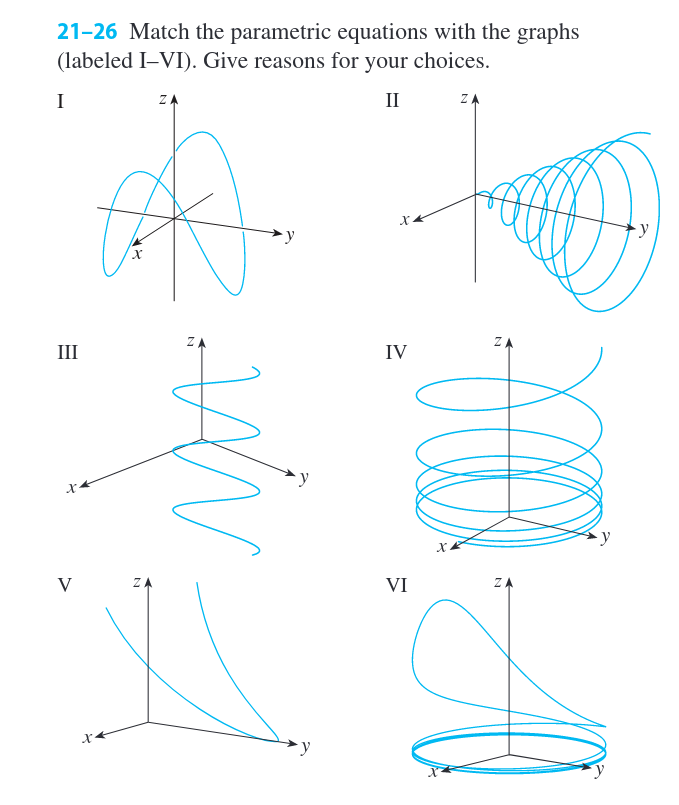
\includegraphics[width=0.7\textwidth]{w5-1.png}
		\end{center}
	\end{figure}

	\begin{figure}[ht]
		\begin{center}
			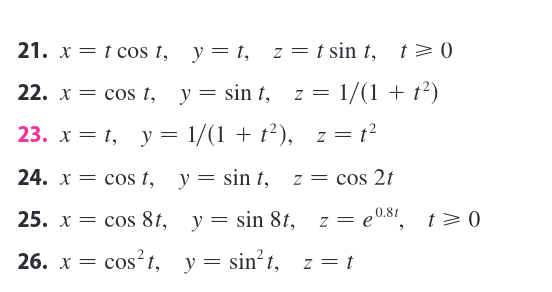
\includegraphics[width=0.7\textwidth]{w5-2.png}
		\end{center}
	\end{figure}


\end{question}


\end{document}
